\chapter{SMT}
\label{ch:smt}

Satisfiability Modulo Theories (SMT) představuje rozšíření klasického problému splnitelnosti booleovských formulí (SAT).
Podstatou SMT je obohacení výrokové logiky o specializované teorie,
mezi něž patří celočíselná aritmetika, aritmetika reálných čísel, teorie bitových vektorů a další.
Označení \uv{modulo theories} vyjadřuje, že splnitelnost se posuzuje vzhledem (modulo) k dané teorii.
SMT nachází uplatnění především v oblasti formální verifikace softwaru a v automatizovaném dokazování~\cite{SMT}.

Mezi nejpoužívanější SMT řešiče patří Alt-Ergo, CVC a Z3.
Tyto řešiče jsou open-source a integrované do obou nástrojů Frama\mbox{-}C i~Stainless.
Přestože mají stejný cíl, liší se v implementaci a algoritmech, které používají.
Každý SMT řešič lze používat samostatně,
ale výhodné je kombinovat několik SMT řešičů najednou, porovnat výsledky a využít silné stránky každého z nich.
Některé úlohy mohou být pro jeden SMT řešič snadno vyřešitelné,
ale pro jiný mohou být složité nebo dokonce neřešitelné,
protože pro daný typ úlohy není řešič naprogramovaný.
Tabulka~\ref{tab:smt-resice} zobrazuje informace o jednotlivých SMT řešičích.
Sloupec programovací jazyk obsahuje jazyk, ve kterém je daný SMT řešič napsaný.
Většina SMT řešičů ale obsahuje API (Application Programming Interface),
pomocí kterého je možné používat daný SMT řešič i v jiných programovacích jazycích.
Všechny SMT řešiče také podporují vstup ve standardním formátu SMT-LIB,
který bude představen v následující kapitole~\ref{sec:smt-lib}.

\begin{table}[H]
    \centering
    \begin{tabular}{|c|c|c|}
        \hline
        \textbf{Název} & \textbf{Rok vydání}  & \textbf{Programovací jazyk} \\
        \hline
        Alt-Ergo       & 2006                 & OCaml                       \\
        CVC4           & 2012                 & C++                         \\
        CVC5           & 2021                 & C++                         \\
        Z3             & 2007                 & C++                         \\
        \hline
    \end{tabular}
    \caption{Základní informace o SMT řešičích}
    \label{tab:smt-resice}
\end{table}

Řešiče SMT zpravidla kombinují hlavní algoritmus pro řešení SAT společně
s~knihovnou podporovaných teorií.
Konkrétně řešič Z3, jehož architektura je znázorněna na obrázku~\ref{fig:z3-block-diagram}, využívá algoritmus DPLL(T)~\cite{Z3Intro},
který bude představen v následující části.
Stejný princip algoritmu DPLL(T) využívají i řešiče CVC4~\cite{cvc4_website} a CVC5~\cite{cvc5_website}.
Alt-Ergo používá algoritmus CC(X) (Congruence Closure parametrized by a theory X)~\cite{AltErgo}.

\begin{figure}[H]
    \centering
    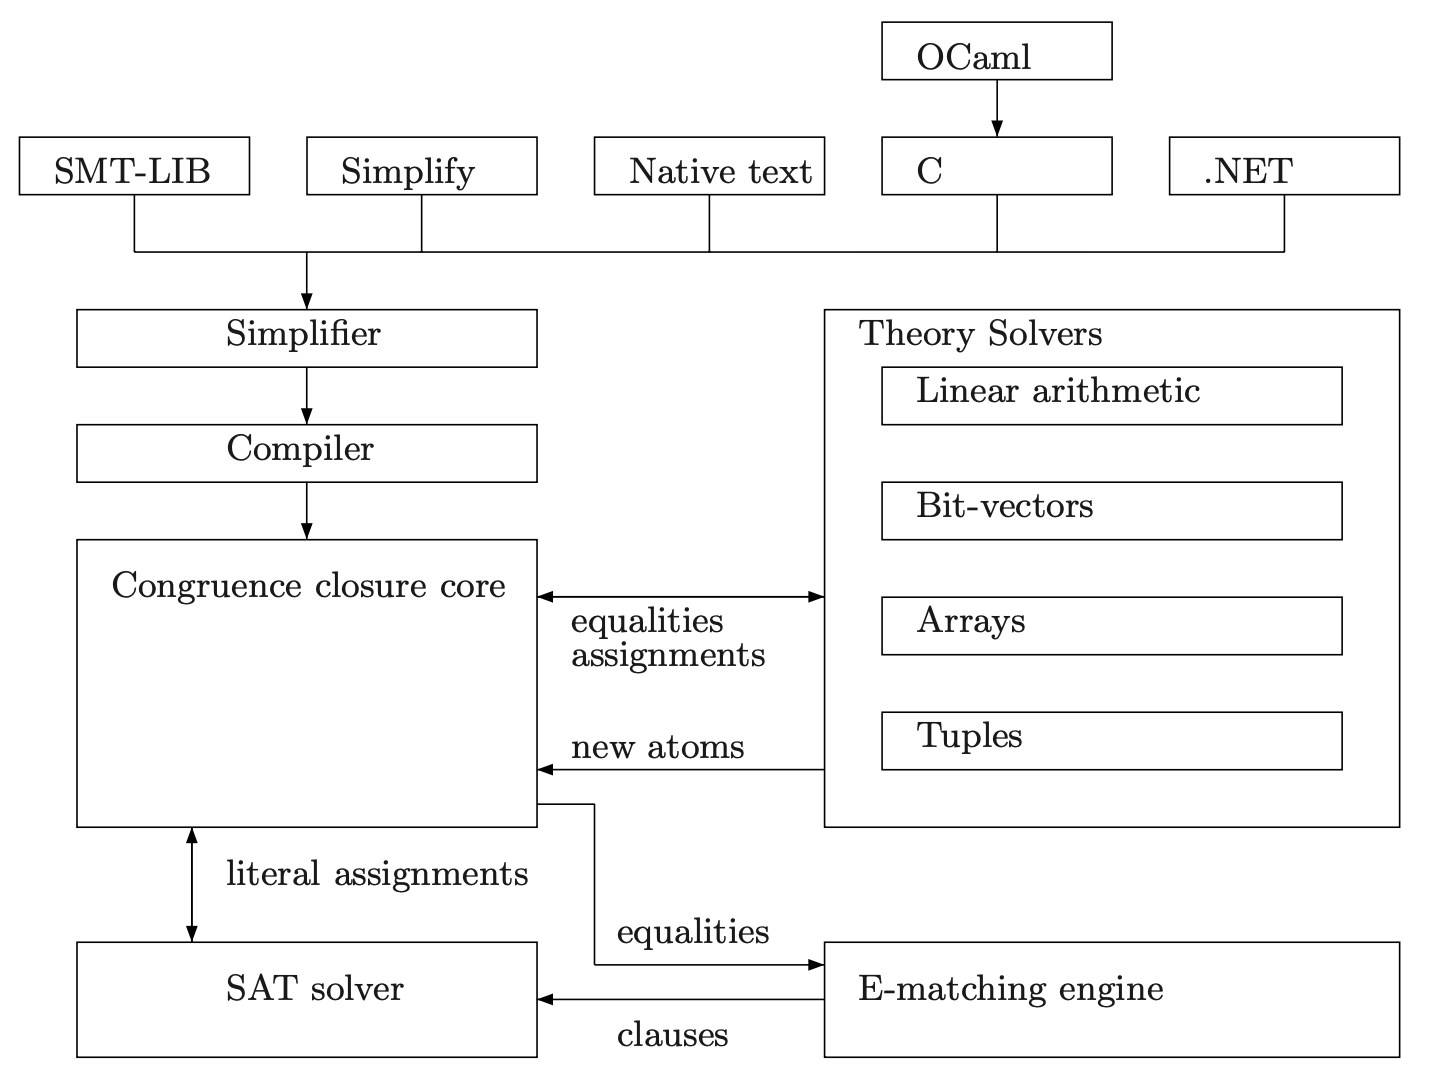
\includegraphics[width=\linewidth]{images/smt-structure}
    \caption{
        Blokový diagram SMT řešiče Z3. \\
        Převzato z článku Z3: An Efficient SMT Solver~\cite{Z3}.
    }
    \label{fig:z3-block-diagram}
\end{figure}

Algoritmus DPLL (Davis-Putnam-Logemann-Loveland) představený roku 1961
je algoritmus pro řešení SAT problémů
založený na rekurzivním prohledávání do hloubky, rozhodování o ohodnocení proměnných a zpětné propagaci (backtracking).
Algoritmus je založen na propagaci jednoduchých důsledků (unit propagation) v případě jednoduchých klauzulí
a rozhodování o ohodnocení proměnných v případě složitějších klauzulí.

Rozšířený algoritmus DPLL(T) zahrnuje teorii T, podporovanou SMT řešičem.
Tento algoritmus se skládá ze dvou částí.
První část je algoritmus DPLL pro SAT, který se stará o generování kandidátních ohodnocení proměnných.
SMT řešič kóduje vlastnosti z teorie T do booleovských proměnných a klauzulí.
Druhá část je SMT řešič dané teorie, který dostává kandidátní ohodnocení proměnných od SAT řešiče a kontroluje logickou konzistenci
v rámci dané teorie.
Tento proces se opakovaně provádí a pokud je nalezena neslučitelnost v SMT teorii,
tak SMT řešič informuje SAT řešič o dané neslučitelnosti pomocí konfliktní klauzule.
Tato klauzule je poté přidána do původní formule a DPLL algoritmus pokračuje v hledání dalšího ohodnocení proměnných
v rozšířené formuli~\cite{DPLLT}.

Následující příklad demonstruje, jakým způsobem SMT řešiče fungují.
Teorie pro tento příklad je lineární celočíselná aritmetika (LIA, Linear Integer Arithmetic).
Vstupní formule pro SMT řešič popisuje tento problém:

\begin{equation*}
    (x \geq 0) \land (x \geq 1 \lor x \leq -1)
\end{equation*}

Tento vstup je nejdříve zakódován do booleovských proměnných a klauzulí.
Konkrétně u tohoto příkladu si SMT řešič zapamatuje mapování

\begin{align*}
    A &= \{ x \geq 0 \} \\
    B &= \{ x \geq 1 \} \\
    C &= \{ x \leq -1 \}
\end{align*}
a vygeneruje formuli pro SAT řešič

\begin{equation*}
    A \land (B \lor C)
\end{equation*}

Tato formule je poté předána SAT řešiči, který se pokusí najít ohodnocení proměnných.
Pomocí jednotkové propagace SAT řešič zjistí, že $A$ musí být pravdivé.
V druhé klauzuli $B \lor C$ se SAT řešič náhodně rozhodne a nastaví $C$ na pravdivé ohodnocení.
Tímto způsobem SAT řešič zjistí, že ohodnocení

\begin{align*}
    A &= \texttt{true} \\
    C &= \texttt{true}
\end{align*}
splňuje danou formuli a přepošle toto kandidátní ohodnocení SMT řešiči.

Pro SMT toto ohodnocení znamená, že musí platit $x \geq 0$ a zároveň $x \leq -1$.
Toto ohodnocení je v rámci teorie LIA neslučitelné, protože $x$ nemůže být zároveň větší než 0 a menší než -1.
SMT řešič tedy informuje SAT řešič o této neslučitelnosti pomocí konfliktní klauzule

\begin{equation*}
    \neg (A \land C) = \neg A \lor \neg C
\end{equation*}
a celá formule pro SAT řešič se tedy změní na

\begin{equation*}
    A \land (B \lor C) \land (\neg A \lor \neg C)
\end{equation*}

Rekurzivním prohledáváním SAT řešič nyní nastaví ohodnocení $B$ na pravdivé,
jelikož by jinak nebylo možné splnit klauzuli $B \lor C$.
Zároveň nastaví $C$ na nepravdivé,
protože je stále $A$ pravdivé a poslední klauzule je splnitelná
pouze pokud je $C$ nastaveno na nepravdu.
A tedy nové kandidátní ohodnocení

\begin{align*}
    A &= \texttt{true} \\
    B &= \texttt{true} \\
    C &= \texttt{false}
\end{align*}
je odesláno pro kontrolu SMT řešiči.

SMT řešič kontroluje pouze pravdivě ohodnocené proměnné $A$ a $B$.
Kombinace těchto proměnných reprezentuje podmínku $x \geq 0$ a $x \geq 1$,
což je v rámci teorie LIA slučitelné.
Jelikož SAT řešič našel ohodnocení proměnných, které splňuje celou formuli
a SMT řešič potvrdil, že toto ohodnocení je slučitelné v rámci dané teorie,
tak lze prohlásit vstupní formuli za splnitelnou v rámci dané teorie.

\section{Standard SMT-LIB}
\label{sec:smt-lib}

SMT-LIB je standardizovaný jazyk pro SMT, který definuje syntaxi a sémantiku pro zápis SMT problémů.
Tento standard byl vyvinut pro usnadnění výzkumu, vývoje a porovnávání různých SMT řešičů.

Od roku 2005 se pravidelně pořádá soutěž SMT-COMP (SMT Competition),
ve které se porovnávají různé SMT řešiče na základě jejich výkonu na různých typech problémů.
Problémy jsou definovány ve formátu SMT-LIB~\cite{SMTCOMP}.

Ukázka~\ref{lst:smt-lib-example} zobrazuje příklad SMT-LIB kódu pro booleovskou formuli

\begin{equation*}
    p \land (p \lor \neg q)
\end{equation*}
kde $p$ a $q$ jsou booleovské proměnné.

\begin{listing}[H]
    \begin{minted}{lisp}
    (set-logic QF_UF)

    (declare-const p Bool)
    (declare-const q Bool)

    (assert (and p (or p (not q))))

    (check-sat)
    (get-model)
    \end{minted}
    \caption{Příklad SMT-LIB kódu pro booleovskou logiku}
    \label{lst:smt-lib-example}
\end{listing}

Pomocí volání funkce \texttt{check-sat} lze zjistit, zdali existuje řešení pro danou formuli.
Pokud ano, SMT-LIB vrátí \texttt{sat}, jinak vrátí \texttt{unsat}.
Pokud je výsledek \texttt{sat}, lze pomocí funkce \texttt{get-model} získat konkrétní hodnoty proměnných, které splňují danou formuli.
Pro tuto formuli byl nalezen model s ohodnocením $p = \texttt{true}$ a $q = \texttt{false}$.
Zvolená teorie je \texttt{QF\_UF} (Quantifier-Free Uninterpreted Functions),
což znamená, že se jedná o logiku bez kvantifikátorů nad neinterpretovanými funkcemi.
Neinterpretované funkce jsou funkce, které nemají žádnou konkrétní interpretaci a jejich význam je dán pouze jejich syntaktickým zápisem.
Konstanty reprezentující proměnné jsou deklarovány pomocí funkce \texttt{declare-const},
což je pouze syntaktický cukr pro neinterpretovanou funkci bez parametrů~\cite{SMTLIB}.

Ukázka~\ref{lst:smt-lib-example-int} zobrazuje příklad SMT-LIB kódu pro celočíselnou aritmetiku.
Konkrétně se jedná o příklad se soustavou dvou rovnic o dvou neznámých.

\begin{align*}
    x + y &= 5 \\
    2x - y &= 4
\end{align*}
kde $x$ a $y$ jsou celočíselné proměnné.

\begin{listing}[H]
    \begin{minted}{lisp}
    (set-logic QF_LIA)

    (declare-const x Int)
    ; syntax sugar for (declare-fun y () Int)
    (declare-const y Int)

    (assert (= (+ x y) 5))
    (assert (= (- (* 2 x) y) 4))

    (check-sat)
    (get-model)
    \end{minted}
    \caption{Příklad SMT-LIB kódu pro celočíselnou aritmetiku}
    \label{lst:smt-lib-example-int}
\end{listing}

Pomocí SMT řešiče lze získat řešení $x = 3$ a $y = 2$.

Pokud bychom měli funkci, která by mohla obsahovat více než jedno řešení,
jako například

\begin{equation*}
    x^2 - 4 = 0
\end{equation*}
mohli bychom interaktivně s SMT řešičem procházet jednotlivá řešení.
Po získání prvního řešení bychom mohli přidat další podmínku, která by vyloučila
první nalezené řešení a pokračovat v hledání dalších řešení.
Tento interaktivní přístup je vhodné naprogramovat, ale výsledné volání SMT řešiče
by vypadalo stejně, jako v následujícím příkladu~\ref{lst:smt-lib-example-sqrt}.

\begin{listing}[H]
    \begin{minted}{lisp}
    (set-logic QF_LIA)

    (declare-const x Int)

    (assert (= (- (* x x) 4) 0))

    (check-sat)
    (get-model)

    (assert (not (= x 2)))

    (check-sat)
    (get-model)

    (assert (not (= x -2)))

    (check-sat)
    \end{minted}
    \caption{Příklad SMT-LIB kódu pro hledání více řešení}
    \label{lst:smt-lib-example-sqrt}
\end{listing}

Tímto postupem nám SMT řešič postupně oznámí dvakrát výsledek \texttt{sat} s modelem pro proměnnou $x$ s hodnotami $2$ a $-2$.
Nakonec oznámí výsledek \texttt{unsat}, což znamená, že neexistuje další řešení a program by měl skončit.
